\documentclass{article}
\usepackage[utf8]{inputenc}
\usepackage[portuguese]{babel}
\usepackage{csquotes}
\usepackage{graphicx}
\usepackage{adjustbox}
\usepackage{lipsum}
\usepackage[backend=biber,autolang=other,bibencoding=utf8,style=alphabetic]{biblatex}
\addbibresource{villard-de-honnecourt.bib}

\title{Villard de Honnecourt, o desenhador}
\date{17 de Dezembro de 2014}
\author{João Távora \\Faculdade de Belas Artes da Universidade de Lisboa}

\begin{document}

\maketitle

\section{Sinopse}

O presente trabalho consiste num estudo premilinar sobre Villard de
Honnencourt, arquitecto francês da primeira metade do séc XIII, a
partir do seu único legado artístico conhecido, um conjunto de notas e
desenhos sobre artes manuais, encadernados pelo próprio Villard num
caderno deixado na loja profissional a que pertencia. O trabalho
debruça-se sobre os aspectos biográfico e artístico evidenciados neste
caderno. O primeiro sustenta-se primariamente num ensaio de Teresa
Frisch \cite{teresa}, e em referências secundárias dele
extraídas. Para o segundo focou-se o livro ``Arte e Ilusão'' de
E.H. Gombrich \cite{gombrich}.

\section{Palavras-chave}

\section{Introdução}

De Villard de Honnecourt sobreviveu um portfólio de 33 folhas de
pergaminho contento desenhos que datam de uma fatia razoavelmente
pequena da primeira metade do séc XII. Os desenhos e notas realizadas
a tinta e pena sobre folhas de pergaminho, guardados hoje em dia na
\emph{Bibliothèque Nationale} em Paris, abarcam uma quantidade
impressionante de temas. A variedade dos assuntos abordados, desde
notas sobre arquitectura, mecanismos de guerra, natureza e figura
humana, tornam difícil a atribuição de um propósito único à obra. A
natureza confusa desta abordagem, intercalando desenho e texto,
intensifica esta dificuldade e valeram-lhe comparações com os
\emph{codices} de Leonardo Da Vinci.

Dado o pouco que se escreveu e se conhece deste arquitecto viajado
pela Europa, é interessante interrogarmo-nos sobre as razões a forma
como esta obra seduz quem sobre ela se debruça. Em primeiro está a
singularidade da obra no seu formato, conteúdo e lugar histórico. Em
segundo lugar, coloca-se o enigma do homem que a escreveu. Na primeira
página, e na primeira pessoa, Villard de Honencourt saúda o leitor e
roga-lhe em primeiro lugar que o recorde e que encontre utilidade nos
conselhos sobre a ``grande arte da construção'', a ``arte do desenho''
e a ``disciplina da geometria''. Em todas as páginas seguintes,
Villard não desaponta. Em cada uma encontram-se vivacidade e
inventividade gráficas fora de série, seja no desenho de flamingos ou
das capelas radiantes de uma catedral cisterciana.

No portefólio de desenhos, Villard fala ao leitor em tom coloquial, e
concentra um entusiasmo informal pelos temas observados e momentos
vividos . A obra tem um carácter concentrado na pessoa no autor, quase
intimista, uma atitude rara na idade média \footnote{Sabemos, por
  exemplo, que o Abade Suger omitiu deliberadamente, dos seus escritos
  sobre a reconstrução da abadia de St. Denis, os nomes dos
  arquitectos e artífices na que nela participaram.}. Talvez por esta
razão fale através dos séculos aos autores contemporâneos.

\section{Aspectos biográficos}

Em \cite{teresa} Teresa Frisch repassa a investigação biográfica sobre
o arquitecto francês. A primeira observação é precisamente sobre o a
apropriação do termo ``arquitecto''. Segundo \cite{pevsner} na idade
média dos séculos XIII e XIV, os termos ``pedreiro'' e ``arquitecto''
designam, do ponto de vista técnico, a mesma actividade, sendo a
distinção feita a partir do nível de especialização e da patente. Da
frequência de desenhos e notas sobre arquitectura, poderemos então
especular, apesar de não haver disso prova directa, que a aprendizagem
de Villard foi sobretudo a de um construtor, que terá começado como
pedreiro, e que gradualmente terá adquirido proiminência e reputação
como executante sobredotado e inteligente. Esta evolução tê-lo-á
levado a encomendas de maior dimensão técnica, artística ou
administrativa, a um melhor salário e a privilégios sociais
exclusivos, como a possibilidade de viajar. \cite{teresa} observa
ainda que os primeiros passos nesta progressão teriam sido mais fáceis
para um jovem nascido numa família de arquitectos distintos.

No caso de Villard, de quem não se sabem data de nascimento ou morte,
o estilo de desenho, e escolha de elementos arquitectónicos e estilo
de desenho coloca o seu período activo no na primeira parte do
séc. XIII. Podemos assumir que terá feito a sua aprendizagem perto de
Honnecourt, aldeia perto de Cambrai na Picardia nortenha, talvez na
abadia cisterciana de Vaucelles. É interessante notar que existe uma
planta do coro desta igreja entre os desenhos do portefólio.

Segundo \cite{teresa} e \cite{hanhloser}, Villard terá desanhado, em
conjunto com outro arquitecto, Pierre de Corbie, o característico
ambulatório com capelas radiantes de uma igreja cisterciana, bem como
a planta do presbitério e uma planta completa de outras duas igrejas
cistercianas. Podemos deste modo assumir que Villard trabalhou para
esta ordem, e que possivelmente terá trablhado na catedral de Cambrai,
numa fase já acançada da sua construção, interrompida em 1231, já que
exprime preocupação pelo estado da mesma, numa página onde se desenham
detalhes da catedral de Reims.

De Reims, Villard viaja para a Hungria, uma viagem que menciona em
várias ocasiões. Não se sabe o propósito profissional desta viagem,
mas admite-se que se tratasse de uma encomenda advinda da sua
associação com a ordem de Cister. A única reminiscência artística da
viagem é um desenho do mosaico da igreja.

Talvez terá sido a caminho da Hungria que Villard realizaou os
desenhos das torres da catedral de Laon, pormenores das fachadas da
catedrais de Chartres de Lausanne.

É geralmente assumido \cite{teresa} que Villard terá regressado da
Hungria antes da invasão tártara de 1241 e que terá passado o resto da
sua vida na Picardia, talvez como mestre de loja \footnote{Por esta
  razão ao portefólio de desenhos compilados e encadernados por
  Villard se chame frequentemente ``livro de loja'' \cite{teresa}}na
igreja de St. Quentin, onde se viria a construir uma das maiores
abadias do séc. XIII viria a ser construida.

\section{O caderno de Desenhos}

A par das competência gráficas, e em grande medida por via destas, o
caderno de desenhos de Villard de Honnencourt revela um homem com um
olhar e mente aguçados, astudo na absorção de conhecimentos,
consciente das teorias artísticas e científicas da época, e dialogante
com estas. Em \cite{teresa}, observa-se ainda que, a julgar pela
diversidade de temas tratados na pequena amostra chegada à
actualidade, as tarefas a que se dedicou terão sido tão numerosas,
diversas e exigentes como aquelas de que fala Vitrúvio no seu tratado
de Arquitectura.

Aquando da encadernação, Villard, que viria a presidir sobre loja
profissional à qual se tinha associado, acrescentou notas e
comentários. Mais tarde, viria a acrescentar desenhos técnicos
relacionados com técnicas de construção, medidas e geometria aplicada
de acordo com as necessidades de uma loja de
pedreiros. \footnote{Posteriormente, outros membros da loja, mais ou
  menos próximos de Villard, acrescentaram outras notas de desenhos ao
  portefólio. Não foram, no entanto, tocadas as observaçãos de
  carácter estético ou a coleção de construções e invenções de
  engenharia.}

Villard abre o portfólio dirigindo-se ao leitor:

\begin{quote} Villard de Honnecourt saúda-vos e exorta todos aqueles
que possam no trabalho ser auxiliados por este livro que rezem pela
sua alma e o recordem. Neste livro poder-se-áo encontrar bons
conselhos sobre a grande arte da construção e engenhos de carpintaria,
e nele encontrareis a arte do desenho [...] e seus princípios, assim
como a disciplina da geometria os requer e os
ensina. \footnote{Tradução livre do autor a partir de \cite{teresa}.}
\end{quote}

\subsection{Forma e função}

Na pequena nota introdutória, Villard explica a função dual da obra:
Em primeiro lugar, adjectivada de ``grande arte'' está a função
prática e profissional da obra. Em segundo lugar está a ``arte do
desenho'' que serve a disciplina da geometria.

A estruturação contém, de forma subtil, uma importante e necessária
hierarquização típica da idade média: os discursos prático-científico
e estético estão sempre subordinados ao discurso religioso. Apesar de
aparecer em último, é no entanto notável que a``arte do desenho''
conste desta enumeração.

Os desenhos de Villard, que \cite{teresa} classifica em seis grupos,
podem agrupar-se de forma mais simples em três: (1) animais, (2)
figura humana e (3) desenhos diagramáticos.

Nesta última categoria, onde se contam os desenhos de arquitectura,
geometria, ornamentação e carpintaria. Prevalece nela a função
diagramática dos desenhos, dos quais subsistem as linhas claras,
firmes e desambíguas inscritas a tinta no pergaminho. Nos comentários
que acompanham prevalece o carácter explicativo com indicações da
apropriação da forma à função:

\begin{quote}
  Quem desenhar fazer um púlpito do qual se possam ler as escritura,
  contemple a melhor maneira de o fazer [...]  \cite{villard, p??}
\end{quote}

\begin{quote}
  Quem desejar fazer uma caixa para o relógio, poderá ver aqui uma
  que vi numa ocasião. \cite{villard, p??}
\end{quote}

\begin{quote} Se desejardes fazer uma asa satisfatória de uma cadeira
de coro verdadeiramente boa, vede esta. \cite{villard, p??}
\end{quote}

\begin{quote} E o andar de cima terá que ter ameias para que ninguém
  possa passar pelo telhado. \cite{villard, p??}
\end{quote}

O desenho diagramático de Villard é irreprensível, com todas as linhas
firmes, uniformes e bem determinadas. Os pormenores tornados claros
apenas quando necessário, recorrendo a sistemas informais, mas
eficazes, de perspectiva.

É interessante verificar que, estritamente dentro do grupo
diagramático, os desenhos são tanto mais exuberantes e imponentes,
quanto mais derivam produto da observação directa (e não de
projecto). Por outras palavras, Villard, plenamento atento à função
está igualmente consciente da forma, e da maneira como esta afecta e
se relaciona com o vazio da página. Alguns desenhos evidenciam um
contacto visual intenso e uma verdadeira empatia pelo modelo
arquitectónico. É o próprio Villard que que assim descreve o seu
desenho de uma janela da catedral de Reims FIGURA. \cite{villard,
  p??}:

\begin{quote}
Contemplai uma das janelas em Reims da [...] nave, assim como são
entre dois pilares. Mandaram-me para as terras de Hungria porque
gostei mais dela. \cite[p. ??]{villard}
\end{quote}

Não só Villard se permite temerariamente dar o seu juízo artístico
como o relaciona directamente com a possibilidade de viajar para a
Hungria. Hans Hahnloser \cite[p. ??]{hahnloser} chama a esta afirmação
``o poleiro do juízo artístico pessoal da alta idade
média''\footnote{No original ``the roost personal artistic judgment of
  the high Middle Ages'' segundo \cite{teresa}. Considerou-se a
  omissão do ``of'' uma gralha.}

\subsection{Geometrização}

Uma das primeiras coisas que salta à vista nos desenhos de figuras
humanas e animais é a sobreposição em muitas delas de figuras
geométricas que acompanham o ritmo. Em \cite{gombrich, p130}, Ernst
Gombrich encontra uma explicação para este fenómeno:

\begin{quote}
  [...] the trick figures [...] included in this album of patterns. One
  could find a parallel for each of these diagrams in modern drawing
  books. Villard and his workmates must have experienced the same
  difficulties and needed the same pschological aids in learning to
  draw as we do.
\end{quote}

A explicação didática de Gombrich e a comparação com a ``massa de
livros que vertem da imprensa ano após ano'' \cite[p. 127]{gombrich} é
certamente admissível. É notável, de facto, como numa figura do topo
de uma das páginas \ref{caras-geometricas} encontramos a famosa
``regra de três'' para a estruturação da anatomia frontal da cara:
mede-se a mesma distância da eminência frontal, à eminência nasal, à
base do queixo. O próprio Villard releva esta função \cite[p. 18,
  verso]{villard}.

\begin{quote}
ici commence la méthode des dessins de portraiture, comme l'art de la
géométrie l'enseigne pour travailler aisément
\end{quote}

No entanto, num prévio trabalho, além de mencionar esta explicação
didática \cite[p. 17]{tavora}, analisou-se também a maneira como a
geometria serve os conceitos de ``massa'' e ``impulso'', ou seja
confere solidez e credibilidade à forma, principalmente à figura
humana \cite[p. 6]{tavora}:

\begin{quote}
  Por outras palavras, a representação de sólidos geométricos no
  espaço é um problema fundamental do desenho, uma abordagem poderosa
  à sua resolução, à qual pode não bastar, por exemplo, o foco
  exclusivo na iluminação tonal ou no contorno. Segundo Hale, um
  artista completo possui um riquíssimo vocabulário de possíveis
  geometrizações da forma, que vai enriquecendo ao longo da vida. O
  artista decide qual o sólido geométrico que mais lhe convém para
  resolver determinado problema. Nos retratos de Drawing
  Lessons... nota-se como a cabeça humana é representada
  alternadamente como oval ou paralelipípedo.
\end{quote}

Nesse trabalho, executado à luz da obra de Robert Beverly Hale
\cite{hale}, artista e pedagogo americano, apenas o que diz
estritamente respeito à ilusão da trimensionalidade não se aplica
directamente aos desenhos de Villard de Honnecourt, que utiliza formas
bidimensionais.

É precisamente esta alternância entre formas soluções geométricas que
se encontra nos desenhos de Villard de Honnecourt. Além da
exprimentação com concepções em círculo e rectângulo, Villard utiliza
uma quantidade notável de variações da concepções em estrela para
representar convincentemente várias figuras humanas.

Estejam as formas em sí explicitamente ou implicitamente
presentes\footnote{Segundo \cite{teresa}, Julius Schlosser ``observa
  claramente'' que as figuras geométricas foram sobrepostas depois de
  concebido o desenho, e não o precedem. Nota-se que tal afirmação não
  exclui que a geometria tenha estado explícita no desenho prévio
  antes da passagem a tinta \cite{calado}, ou simplemenente na mente
  do desenhador.}, a geometrização é a pedra de toque do desenho de
raíz europeia e Villard esgrime uma observação perspicaz quando
saliente a relação bidirectional entre o desenho e a geometria.

\begin{figure}
\centering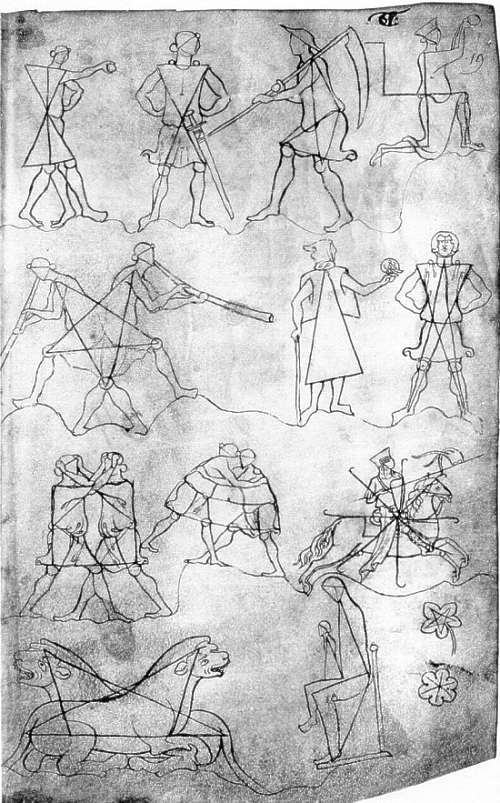
\includegraphics[height=0.6\textheight,keepaspectratio]
                          {images/villard-figuras-solidas.jpg}
  \caption{Página do portfólio de Villard De Honnecourt}.
  \label{fig:villard-figuras-solidas}
\end{figure}

\subsection{O referente ``du vif''}

De todo o caderno de desenhos de Villard de Honnecourt, recaem
invariavelmente as atenções de qualquer autor sobre a página onde se
representa um leão e um ouriço \cite[p. 20]{villard}. O desenho do
leão, que ocupa quase toda a página, é claramente estilizado,
particularmente no rosto. A perplexidade que sugere a legenda
subsequente, em que Villard diz que o desenho foi realizado à vista e
do natural, só é comparável àquela com que o rosto do leão parece
fitar o leitor (\cite[p. 24, verso]{villard} e\ref{villard-leao}):

\begin{quote}
  voici un lion [...] et saves bien qu'il fut contrefait du vif
\end{quote}

Ernst Gombrich, que em \cite{gombrich} analisa com detalhe a relação
entre a finalidade esquemática e ilusória da arte através da história,
adverte para uma leitura correcta do termo ``du vif'', que teriam para
Villard um significado muito diferente do que têm para um observador
contemporâneo. Villard só poderia ter querido dizer que desenhou o seu
\emph{esquema} na presença do Leão. \cite[p. 68]{gombrich}

Para Gombrich, o esquema que o artista medieval desenha \emph{é} a
imagem, sendo para que o artista pós-medieval, ele é o ponto de
partida para correcções. \cite[p. 68]{gombrich}

A partir \cite{teresa}, chegamos a uma citação de \cite{schlosser},
que comunica uma interpretação igualmente cautelosa:
 \begin{quote}
  [...] without doubt Villard did not intend to dissemble when quite
  clearly he did not draw from nature, for to him 'nature' meant
  something different from what it means to us; for a man of the
  Middle Ages it was impossible to consider as meaningful anything but
  the idea, the concept, behind the appearance of things. The natural
  form was like soft wax which had to yield to the artistic invention.
 \end{quote}

O artista medieval tentar representar o particular, e preocupa-se com
o universal. Villard não deseja comunicar a forma \emph{daquele} leão,
mas sim a própria ideia de leão. Em \cite{gombrich}, observa-se por
diversas vezes que esta é a subordinação possível à teoria de arte
platónica vigente na época. Derivando directamente um exemplo do livro
décimo d'\emph{A República} de Platão, ao pintar um aspecto
particular, o pintor está três graus afastado da realidade. O domador
e tratador do leão, cujo método Villard também se esforça por
descrever nas páginas seguintes, estará mais próximo da
realidade.

Em \cite{teresa} observa-se que as figuras de Villard, ainda que no
estilo artístico vigente, têm todas proporções elegantes and noble
proportions and are eloquent in their gestures.

\cite{gombrich} ``How much of his actual observation he allowed to
enter into the picture''

Exemplo do homem de barbas. Imediatismo/espontâneadade na escolha do
lugar geométrico da figura na folha. Exmemplo dos pássaros. Exemplo do
veado.Procura. Ténues linhas auxiliares.

\section{Conclusão}

Obra entusiasmada sobre o desenho. Investigação sobre a arte de
desenhar.

Especulação: Primeiros sintomas de uma emergência do desenho como
disciplina independentente e da função artística como autónoma num
contexto profissional e social florescente.

\printbibliography[heading=bibliography,title={Bibliografia},type=book]
\printbibliography[heading=subbibliography,title={Reproduções},type=artwork]

\end{document}
